\chapter{Probabilistic Score}
\label{chap4}
This paper proposes a departure from the previous cost function definitions, looking instead at using a probabilistic model to directly estimate the likelihood of two edges matching.
\section{Motivation}
A pervasive problem with the cost functions discussed above is that their design is ad hoc and relies on hand-picked values based on the authors' empirical observations. For instance, in \cite{P1} the authors have to decide on the size of the Gaussian window they employ, on the weights to assign to the pixels that fall within that window and on a suitable value for their threshold function. All these parameters are given a static value but, since they are dependent on the source document, the authors would need to manually find different values for each class of documents. In \cite{P2} the authors not only face all of the above problems, but also have to decide on a threshold value for their row comparison and on another threshold regarding the minimum amount of black pixels that an edge must have in order for its matches to be considered relevant. 

This ad-hoc formulation suffer from several impediments which the probabilistic method manages to avoid or at least ameliorate: \\
\begin{table}[H]
  \centering
  \begin{tabular}{p{0.5\textwidth} | p{0.5\textwidth}}
  \toprule
  Cost function & Probabilistic score function \\
  \midrule
Relies on the values the authors hand-picked for their particular dataset. & Learns a new document's pixel distribution by analysing the shreds it is given.\vspace{1.5em} \\
Cannot be easily combined with a different similarity function. & Can be easily composed with any similarity function that produces a probability. Several such functions already exist, such as the optical character recognition based system proposed in \cite{P8}). \\ 
  \bottomrule
  \end{tabular}
  \label{tab:costScoreComp}
\end{table}
\begin{table}[H]
  \centering
  \begin{tabular}{p{0.5\textwidth} | p{0.5\textwidth}}
  \toprule
  Cost function & Probabilistic score function \\ 
  \midrule
Difficult to evaluate results of the function since the numbers outputted are meaningless, only the order of the results matters. & The scores returned are estimated probabilities of a match, so the calibration of the method can be easily checked by comparing estimated and observed probabilities. \vspace{1.5em} \\ 
Cost is additive and must therefore be normalized relative to the sum of lengths of the matching edges. & All scores are normalized probabilities, so length of edges or number of edges matching is irrelevant (see Figure \ref{fig:norm}).  \\ 
  \bottomrule
  \end{tabular}
  \label{tab:costScoreComp}
\end{table}
\begin{figure}[H]
        \centering
        \begin{subfigure}[b]{0.49\textwidth}
                \centering
                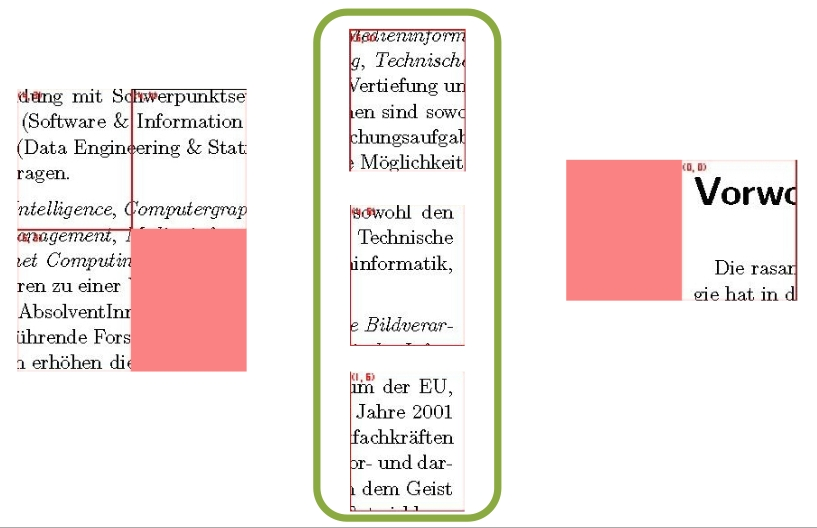
\includegraphics[width=\textwidth]{normPres1}
                \caption{Here we are trying to place one of the 3 shreds in the green rectangle into one of the two red slots. We want to identify the best of the 6 possible placements.\vspace{2\baselineskip}}
        \end{subfigure}
        ~ 
        \begin{subfigure}[b]{0.49\textwidth}
                \centering
                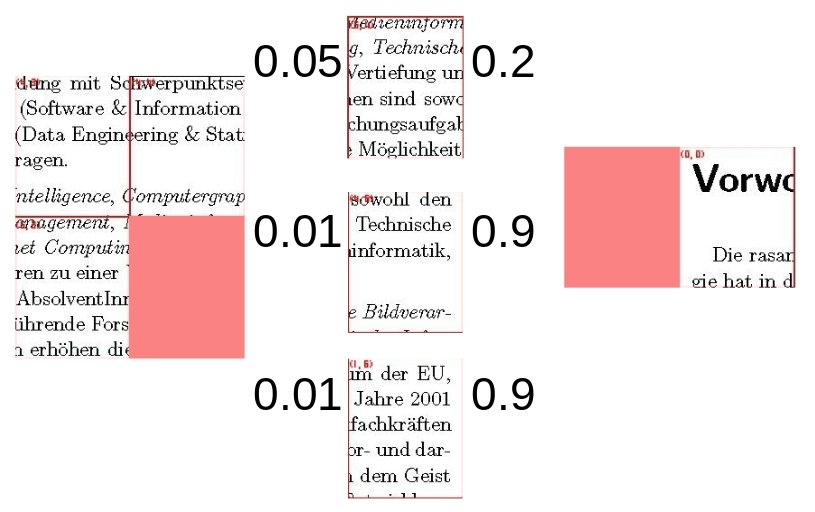
\includegraphics[width=\textwidth]{normPres2}
                \caption{The raw scores are shown. The scores for the left slot are lower since it has two neighbouring edges and therefore more probabilities to multiply together. For the right slot, two of the edges would give a ``white on white" match and therefore a very large score of 0.9.}
        \end{subfigure}
        ~ 
        \begin{subfigure}[b]{0.49\textwidth}
                \centering
                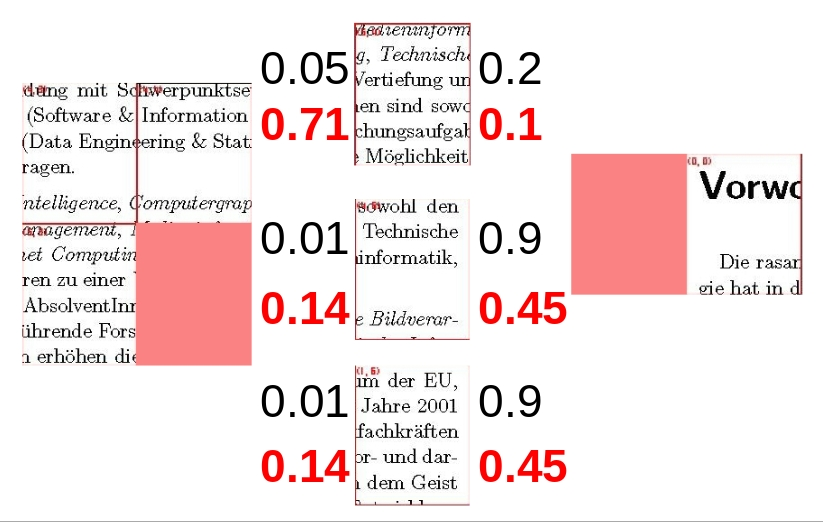
\includegraphics[width=\textwidth]{normPres3}
                \caption{Normalized scores shown in red. Number of pixels multiplied is irrelevant since the scores for each slot must sum up to 1. Probability mass for ``white on white" matches is split between the two possible matches, thus making it less likely that any of them will be picked.}
        \end{subfigure}
        ~ 
        \begin{subfigure}[b]{0.49\textwidth}
                \centering
                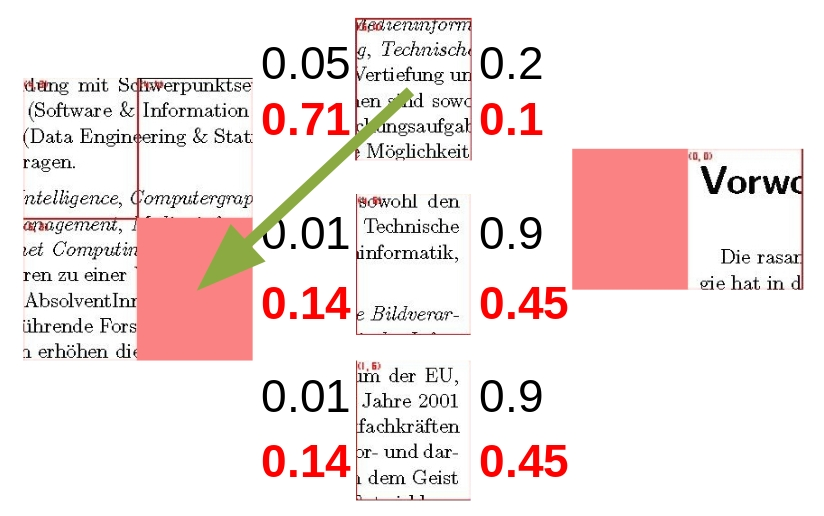
\includegraphics[width=\textwidth]{normPres4}
                \caption{The best placement is shown. Intuitively, this placement is best because its raw score is significantly larger than any of its competitor's. This score distribution means that this placement is the most likely to be correct.\vspace{1\baselineskip}}
        \end{subfigure}
        \caption{Properties of normalization. Both the issue with the varying number of pixels and the ``white on white" matches are solved by normalizing. In contrast, previous methods \cite{P1,P2} had to employ ad-hoc heuristics to address these problems.}
        \label{fig:norm}
\end{figure}
Additionally, as will be shown in Section \ref{chap4Eval}, the probabilistic score outperforms all previously formulated scoring functions.

Lastly, the effectiveness of probabilistic models, when applied to text data, has been repeatedly shown. Pixel prediction goes back to systems such as the 1981 JBIG lossless compression ISO standard (which tried to predict the value of a pixel using several features including 6 of its neighbours \cite{P3}) and is still employed in today's state of the art encoders \cite{P4}. 

\section{Description}

To the best of our knowledge, a probabilistic scoring function has never been previously used in this domain. We therefore choose to restrict ourselves to a relatively simple probabilistic model which can be used as a benchmark for future, more complex, approaches.

When looking at a proposed match, we try to estimate the probability that a candidate pixel is correct given several of its neighbouring pixels (called the candidate pixel's ``context", see Figure \ref{fig:probContext}). We refer to this conditional probability as \(\Pr( p \mid C(p,E_x) )\), where \(C(p,E_x)\) is the context of pixel $p$ when placed next to edge $E_x$. Ideally we'd want to learn these conditional probabilities by analysing the original document, which we obviously don't have access to. However, relatively few pixels are destroyed when shedding a document and we can assume that the ones that are destroyed are uniformly distributed over the space of contexts. Therefore the average distribution of pixels within the shreds will, in general, be a close approximation to the distribution of those in the original document. This similarity means that we can get a good estimate of the needed probabilities by obtaining the probabilities for each individual shred and then averaging them over all shreds.

\begin{figure}[h]
\centering
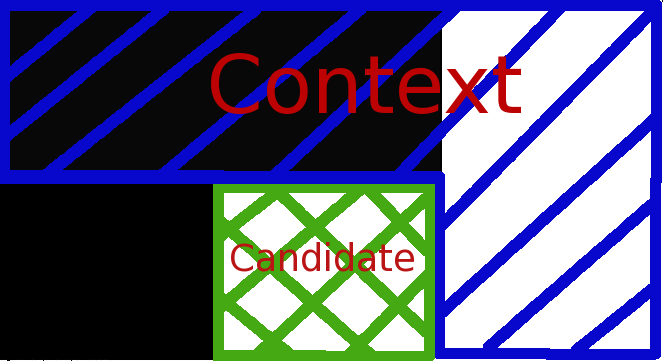
\includegraphics[width=0.8\textwidth]{context}
\caption{This shows a proposed match between the top 3 and the bottom 3 pixels. The model estimates the probability that the candidate pixel is white based on the four context pixels}
\label{fig:probContext}
\end{figure}

\clearpage
\subsection{Edge likelihood}

Once we obtain the conditional probabilities by analysing our shreds, then the raw probability of two edges matching can be calculated by sliding the context down the proposed edge and multiplying all the individual candidate pixel probabilities (see Figure \ref{fig:sliding}). 
\begin{figure}[h]
        \centering
        \begin{subfigure}[b]{0.49\textwidth}
                \centering
                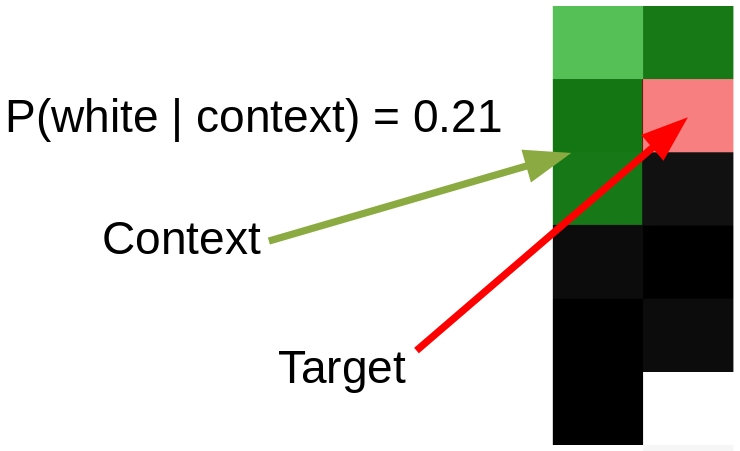
\includegraphics[width=\textwidth]{sliding1}
        \end{subfigure}
        ~ 
        \begin{subfigure}[b]{0.49\textwidth}
                \centering
                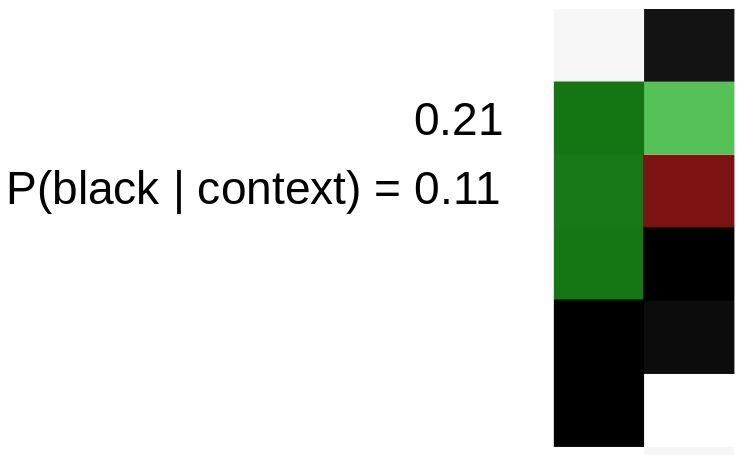
\includegraphics[width=\textwidth]{sliding2}
        \end{subfigure}
        ~ 
        \begin{subfigure}[b]{0.49\textwidth}
                \centering
                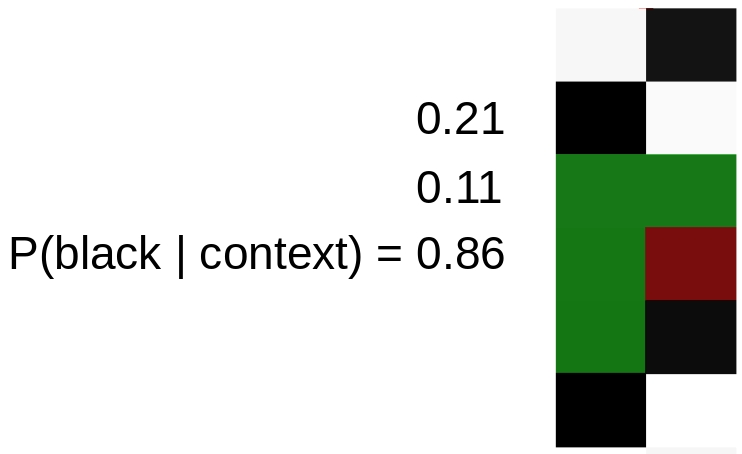
\includegraphics[width=\textwidth]{sliding3}
        \end{subfigure}
        ~ 
        \begin{subfigure}[b]{0.49\textwidth}
                \centering
                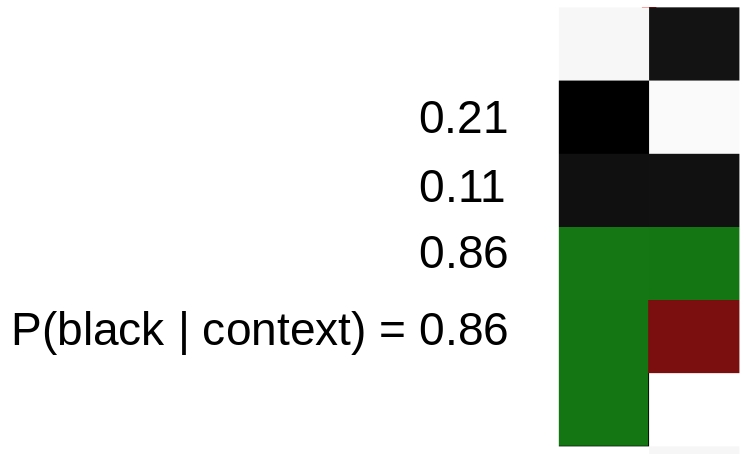
\includegraphics[width=\textwidth]{sliding4}
        \end{subfigure}
        ~
        \begin{subfigure}[b]{0.49\textwidth}
                \centering
                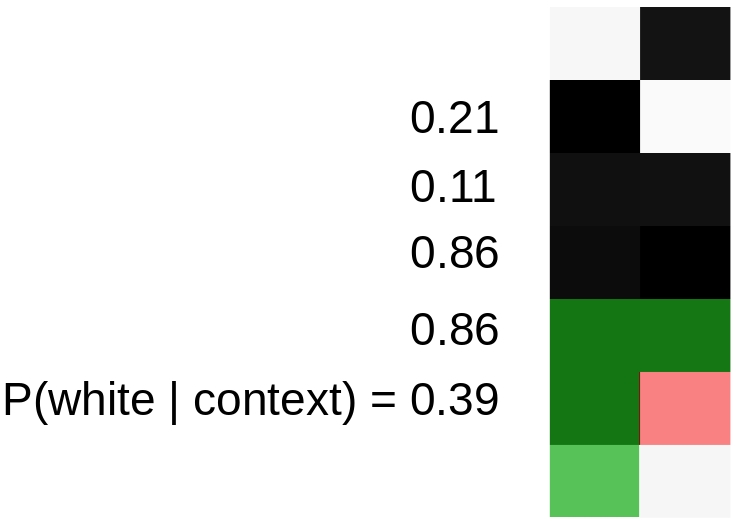
\includegraphics[width=\textwidth]{sliding5}
        \end{subfigure}
        ~ 
        \begin{subfigure}[b]{0.49\textwidth}
                \centering
                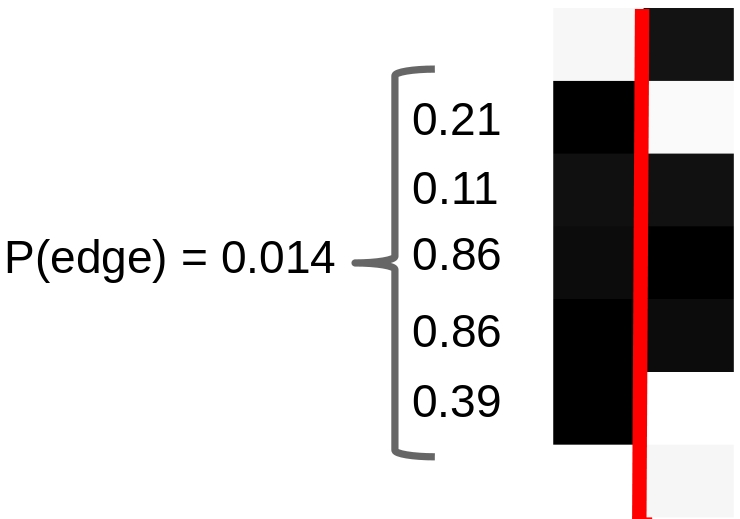
\includegraphics[width=\textwidth]{sliding6}
        \end{subfigure}
        \caption{The context slides down the proposed edge calculating a series of target pixel probabilities. All of these are then multiplied together to give the raw edge probability.}
        \label{fig:sliding}
\end{figure}

That is to say, if we have a proposed matching between edge \(E_1\) and edge \(E_2\), and \(E_1^x\) represents the $xth$ pixel on edge 1, then we would estimate the joint probability of the pixels in the two edges as being: \[\Pr(Pix(E_1),Pix(E_2)) = \prod_{i=1}^{len(E_2)} \Pr(E_2^i \mid C(E_2^i,E_1))\] A problem arises though, because the shape of the context prohibits us from taking the conditional probability for the first and last few pixels (depending on the length of the context). For these the best we can do is assign them the prior probability, \(\Pr(p)\), which is also extracted from the data simply by counting the proportion of white and black pixels. Therefore, when using the context of size 4 shown in Figure \ref{fig:probContext}, the edge probability will actually be: \[\Pr(Pix(E_1),Pix(E_2)) = \Pr(E_2^1) \Pr(E_2^{len(E_2)}) \prod_{i=2}^{len(E_2)-1} \Pr(E_2^i \mid C(E_2^i,E_1)) \]

\subsection{Normalization}\label{sect:norm}
The above, while being a good measure of the joint probability of pixels on an edge, is a function that will tend to decrease as $len(E_2)$ increases. The function will therefore tend to prefer shorter edges with less probabilities to multiply. Luckily, using probabilities gives us one more piece of information here. In the original file, every edge of every shred has only one correct match, since no two shreds are superimposed. Therefore, we know that the sum of the probabilities of all matches along one edge should sum up to one. In technical terms, if \(S_E\) is the set of all edges and \(Pr(E_1,E_2)\) is the probability that edges $E_1$ and $E_2$ match, then: \[\forall E_a \sum_{E_x \in S_E} \Pr(E_a,E_x) = 1 \] To obtain the edge probabilities that satisfy this constraint, the previous pixel probabilities are normalized along every edge. After the normalization, the preference for shorter edges is eliminated and the probabilities for different edges and pieces can be directly compared regardless of local features such as a particular edge length. Therefore, accounting for the normalization process, the final definition becomes\footnote{There actually is a further problem with the presented formula, namely that it doesn't account for edges belonging to the same piece. If \(E_1\) and \(E_2\) both belong to the same shred then obviously the probability that they match is 0 since a shred can't be in 2 places at once. This extra complication is ignored in the mathematical formalism for reasons of clarity}:  \[ \Pr(E_1,E_2) = \frac{\Pr(E_2^1) \Pr(E_2^{len(E_2)}) \prod_{i=2}^{len(E_2)-1} \Pr(E_2^i \mid C(E_2^i,E_1))}{\sum_{E_x \in S_E} \Pr(E_x^1) \Pr(E_x^{len(E_x)}) \prod_{i=2}^{len(E_x)-1} \Pr(E_x^i \mid C(E_x^i,E_1)) } \]


The normalization discussed above has an additional property, which ends up mitigating the predisposition towards whitespace that some of the other cost functions suffer from. The property in question is that if \(E_1\), \(E_2\) and \(E_3\) are very similar or identical edges then they will have less chance of being picked as the best match because the available probability mass of any match will be split equally among the 3 of them. Formally, if \(I_{E_x}\) is the set of edges identical to \(E_x\) then: \[\forall E_a \Pr(E_a,E_x) \leq \frac{1}{\mid I_{E_x} \mid}\] Since there are usually several white edges floating around in the edge set at any time, the above property ends up naturally discounting them without the need for any ad hoc heuristics (see Table \ref{tab:normalization} for a typical situation and Figure \ref{fig:sliding} for an additional illustration). To further discount the white on white matches we can introduce dummy white pieces into the shreds pool.

\begin{table}[h]
  \centering
  \begin{tabular}{|c|c|c|c|c|c|c|}
    \hline
    & \multicolumn{3}{|c|}{Raw probabilities} &  \multicolumn{3}{|c|}{Normalized probabilities} \\
    \cline{2-7}
    & Edge 3 & Edge 4 & Edge 5 & Edge 3 & Edge 4 & Edge 5 \\
    \hline
    Edge 1 & 0.90 & 0.90 & 0.20 & 0.45 & 0.45 & 0.10 \\
    \hline
    Edge 2 & 0.10 & 0.10 & 0.50 & 0.14 & 0.14 & 0.71 \\
    \hline
  \end{tabular}
  \caption{Here Edge 1, 3 and 4 are all white and as such have a very good raw score when matched together. After normalization however, the match between edge 2 and 5 is considered a better bet than any match containing edge 1, as edge 1's probability mass is distributed equally among the identical edges 3 and 4.}
  \label{tab:normalization}
\end{table}

\subsection{Learning}
Given the above descriptions, the problem of calculating the probability of any two edges matching can be reduced to the problem of estimating \(\Pr( p \mid C(p,E_x) )\) for an arbitrary pixel and its context. Depending on the size of the context, various machine learning methods could be used to accomplish this task. However, if the context is of the form shown in Figure \ref{fig:probContext}, then a simple exhaustive exploration of the context space becomes a possible solution. If the context is of size 4, as above, and we are working on black and white documents, then there are only \(2^4 = 16\) possible contexts. Since the number of contexts we can sample is directly proportional to the pixel count of the source image, for an average one page document, the number of observations will exceed 1 million. In practice this means that all 16 possible contexts are well represented in the document (a document where any of the contexts had less than 250 observations hasn't yet been encountered).

Of course the fit to the data will be limited by such a small context, however care must be taken when extending the context as it can easily lead to over-fitting. For instance using a context of size 7 instead of 4 usually leads to having several contexts with a number of observations in the single digits. Such values can, of course, not be trusted. Therefore it seems necessary to use more sophisticated methods in conjunction with a larger context. 

One such attempt was made by using neural networks. Different architectures were tried, with both contexts of size 4 and 7, however no significant difference was found when compared with the above direct estimation. It's likely that a context of 7 was still too small for the neural networks to manage to gain an advantage over direct estimation. Therefore the neural networks were abandoned as the longer training time could not be justified on the small contexts used in this method. If, however, we were to extend the score to use a significantly larger context or an altogether different and more complex probabilistic model, then more involved learning methods would likely prove essential. 

\section{Evaluation}
\label{chap4Eval}
The evaluation measures used here work by comparing the edges predicted by the algorithm to the real edges. In order to obtain the predicted edges, for every edge, we simply take the most likely pair edge. If \(PredMatch(E_a)\) is a function that returns \(E_a\)'s predicted match, then:
\[PredMatch(E_a) = \arg\max_{E_x} \Pr(E_a,E_x) \]

\subsection{Comparison with Gaussian cost functions}
In order to perform this comparison, a function \(CorrMatch(E_a)\) is defined, which returns the correct match for edge $E_a$. With this function we can define the \(score(E_a)\) function as:
\[
score(E_a) =
\left\{
	\begin{array}{ll}
		1  & \mbox{if } CorrMatch(E_a) = \arg\max_{E_x} \Pr(E_a,E_x) \\
		0 & \mbox{otherwise } 
	\end{array}
\right.
\]
However, there's a mistake here. The problem is that \(\arg\max_{E_x} \Pr(E_a,E_x)\) is not guaranteed to return a single element. What we really need to check for then is \( CorrMatch(E_a) \in \arg\max_{E_x} \Pr(E_a,E_x) \). 

This change allows for multiple maximum likelihood matches, but doesn't account for the increased probability that the correct edge is within the predicted set by chance. In the extreme case, if the probability score returned the same value for every edge, then this scoring function would judge any pairing as correct. The solution is to discount the score based on the size of the predicted set (which also makes intuitive sense, since when a search is actually performed, if there are multiple matches with the same probability, the search will simply have to pick one at random). The final score function is:
\[
score(E_a) =
\left\{
	\begin{array}{ll}
		\frac{1}{\mid \arg\max_{E_x} \Pr(E_a,E_x) \mid}  & \mbox{if } CorrMatch(E_a) \in \arg\max_{E_x} \Pr(E_a,E_x) \\
		0 & \mbox{otherwise } 
	\end{array}
\right. 
\]
Therefore the proportion of correctly predicted edges (where \(S_E\) is again the set of all edges) is:
\[
predictedCorrect = \frac{\sum_{E_x \in S_E} score(E_x)}{\mid\left\{E_a \mid CorrMatch(E_a) \in S_E\right\}\mid }
\]
Here the denominator is just counting the number of edges that actually have matches. This is necessary because using \(\mid S_E \mid \) instead would also count the outer edges which have no correct match.

Calculating analogous measures for the cost functions defined in \cite{P1} and \cite{P2} allows us to compare the three methods and shows the probabilistic score as having a relatively consistent advantage\footnote{In the presented graph, the advantage only manifests on samples with more than 50 shreds. The performance on the small cases is very volatile, causing the results of the methods to vary from document to document. The performance on the larger instances is, however, consistently in favour of ProbScore.} over the other functions (see Figure \ref{fig:costComp}).

\begin{figure}[h]
\centering
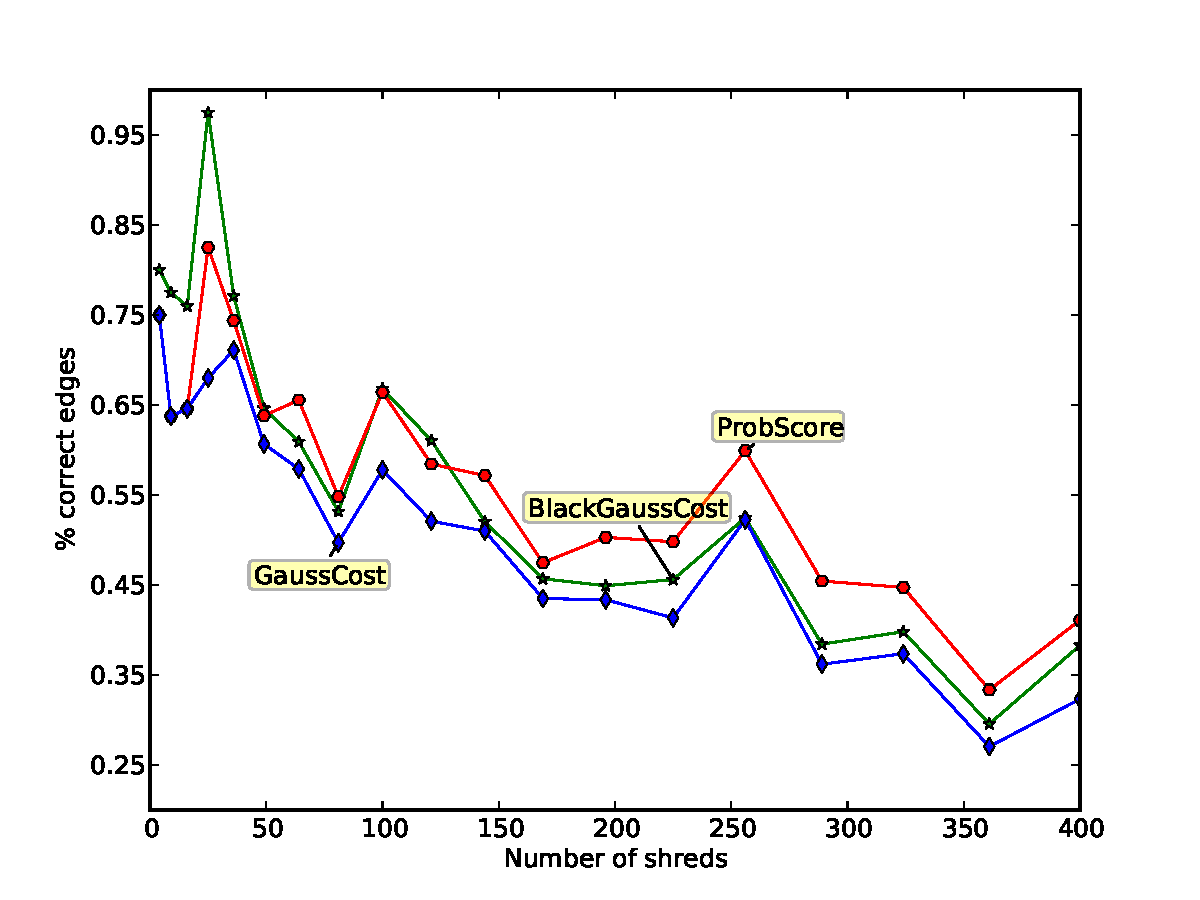
\includegraphics[width=\textwidth]{costComp}
\caption{The probabilistic score has better results on medium and large instances than the cost functions presented in \cite{P1} (GaussCost) and \cite{P2} (BlackGaussCost)}
\label{fig:costComp}
\end{figure}

\subsection{Validity of predicted probabilities}
As mentioned in the Motivation, there is another (perhaps more natural) evaluation that we can perform. Namely comparing the predicted and observed probabilities for our predicted edge matches. The observed probabilities are calculated exactly as in the previous section, and the predicted probabilities are recorded for every predicted match. 

The formula $bucket = \lfloor prob * 10 + 0.5\rfloor$ is used to place the predicted probabilities into one out of a total of 10 buckets. The observed and predicted probabilities are then averaged within each bucket, and the process is repeated for different number of shreds. The resulting graph is Figure \ref{fig:probComp}.
\begin{figure}[h]
\centering
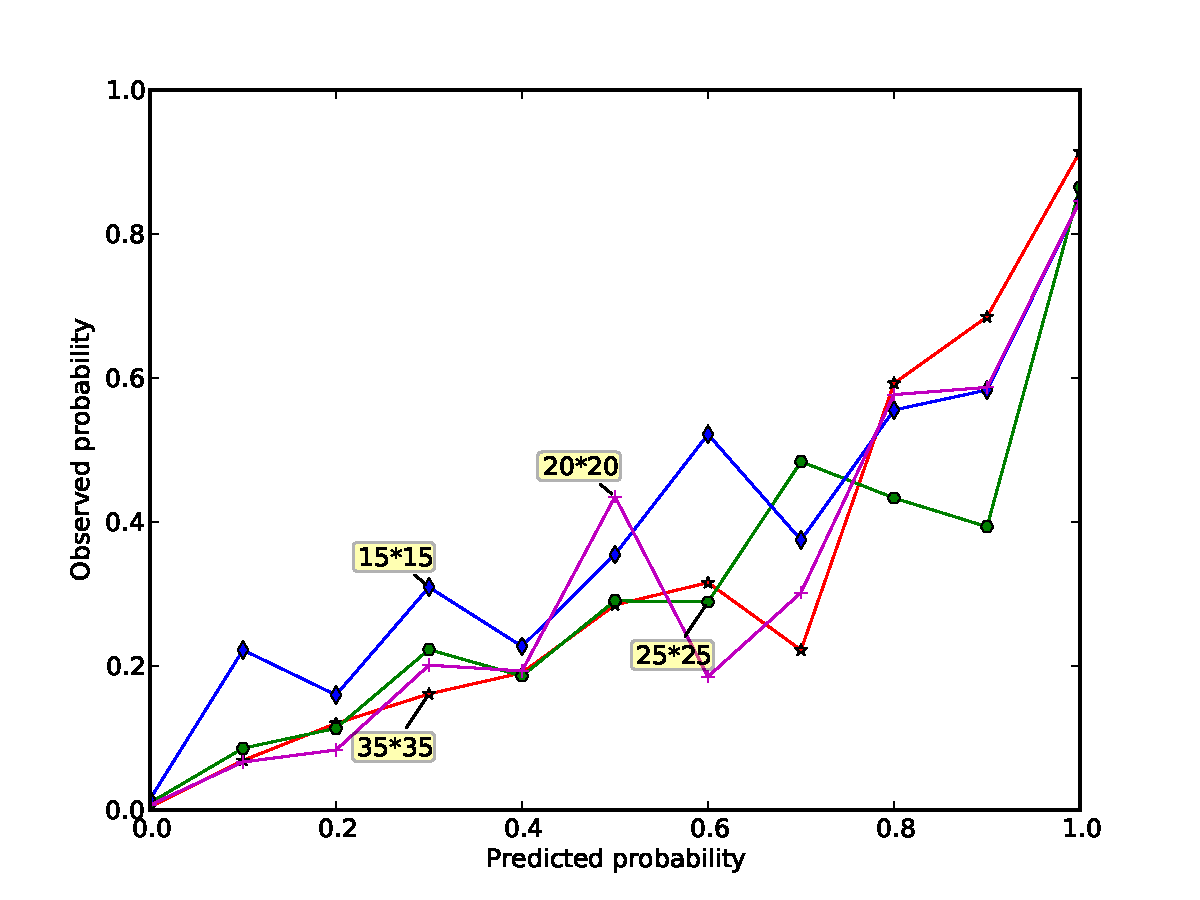
\includegraphics[width=\textwidth]{predObsProb}
\caption{The labels show the number of cross-cut shreds. As the number of shreds increases the relationship between the predicted and observed probability degrades. However the overall shape of the curve is still generally increasing, so a higher predicted probability will usually translate into a higher observed probability and for large predicted probabilities the method is quite accurate}
\label{fig:probComp}
\end{figure}

\subsection{Robustness}
\label{chap4Rob}
Another important aspect worth evaluating is the robustness of the method. When used in real life situations it is unlikely that documents will always be high-resolution, perfectly cut into shreds and completely smudge-free. In order to test this, the results obtained on an image are compared to those obtained when various types of noise are added to the image. 

The types of noise analysed are: downsampling, flipping random pixels and shuffling random pixels around their original position (see Figure \ref{fig:noiseTypes}). 

\begin{figure}[H]
        \centering
        \begin{subfigure}[b]{0.4\textwidth}
                \centering
                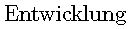
\includegraphics[width=\textwidth]{EntOrig}
                \caption{Original image}
        \end{subfigure}
        ~ 
        \begin{subfigure}[b]{0.4\textwidth}
                \centering
                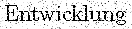
\includegraphics[width=\textwidth]{EntNoise}
                \caption{10\% of bits are randomly flipped}
        \end{subfigure}
        ~ 
        \begin{subfigure}[b]{0.4\textwidth}
                \centering
                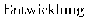
\includegraphics[width=\textwidth]{EntDown}
                \caption{The image is downsampled by a factor of 1.5}
        \end{subfigure}
        ~ 
        \begin{subfigure}[b]{0.4\textwidth}
                \centering
                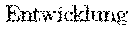
\includegraphics[width=\textwidth]{EntSpread}
                \caption{Pixels are randomly shuffled to one of their neighbours}
        \end{subfigure}
        \caption{How one word of the image is modified by the various types of noise}
        \label{fig:noiseTypes}
\end{figure}

The score evaluation is run on the original and modified documents, and the results are shown in Figure \ref{fig:robustness}. 

\begin{figure}[H]
\centering
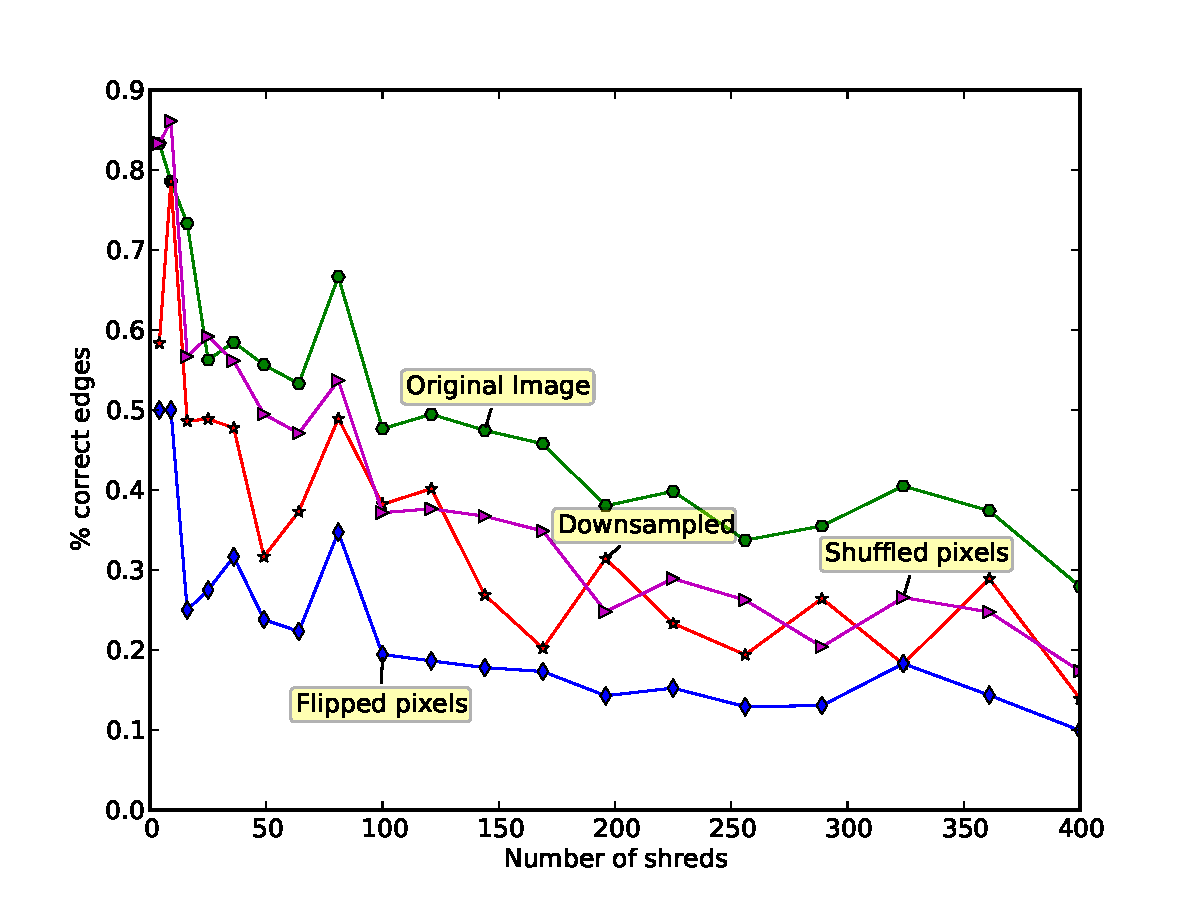
\includegraphics[width=\textwidth]{robustness}
\caption{Degradation of performance between original image and 3 noisy images}
\label{fig:robustness}
\end{figure}

Since the probabilistic scoring function is unique for each document, as it is trained on the noisy shreds, we'd like to see if this gives it an advantage when compared to the stationary Gaussian. Therefore, the probabilistic scoring function is compared with the best Gaussian alternative on all types of noise in Figure \ref{fig:robComp}. As expected some performance degradation is observed in all cases. It is interesting to note that the largest reduction in performance is caused by the random pixel flipping. This can be explained by the fact that the other types of noise are restricted by the existing structure of the document, if you have a section of white pixels, neither downsampling nor shuffling can introduce a black pixel into it. The algorithm seems to suffer more from the unrestrained randomness exhibited by the flipping. The good news is that in real life scenarios most noise should not be completely random and we'd expect it to be more similar to the downsampling and shuffling types of noise than to the pixel flipping.

\begin{figure}[h]
        \centering
        \begin{subfigure}[b]{0.49\textwidth}
                \centering
                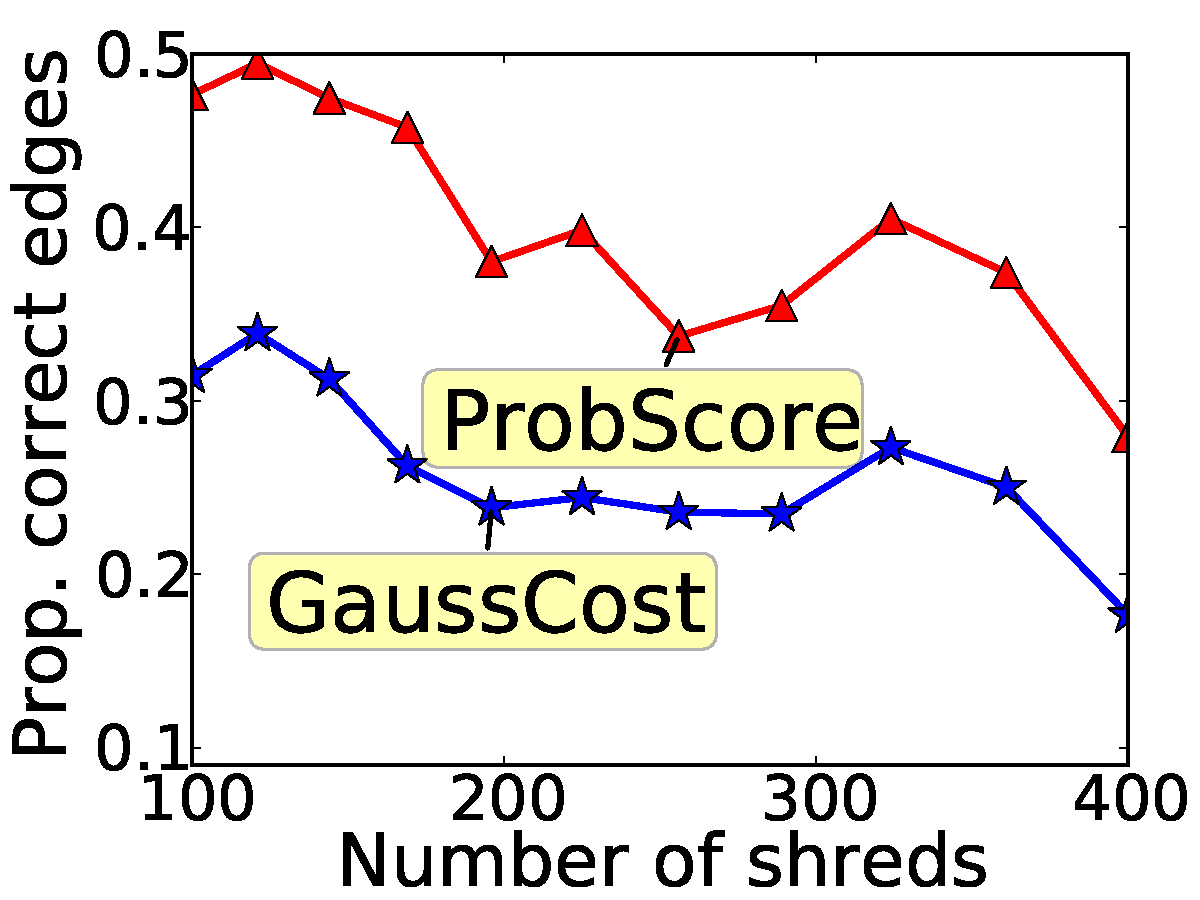
\includegraphics[width=\textwidth]{origComp.pdf}
                \caption{Original image}
        \end{subfigure}
        ~ 
        \begin{subfigure}[b]{0.49\textwidth}
                \centering
                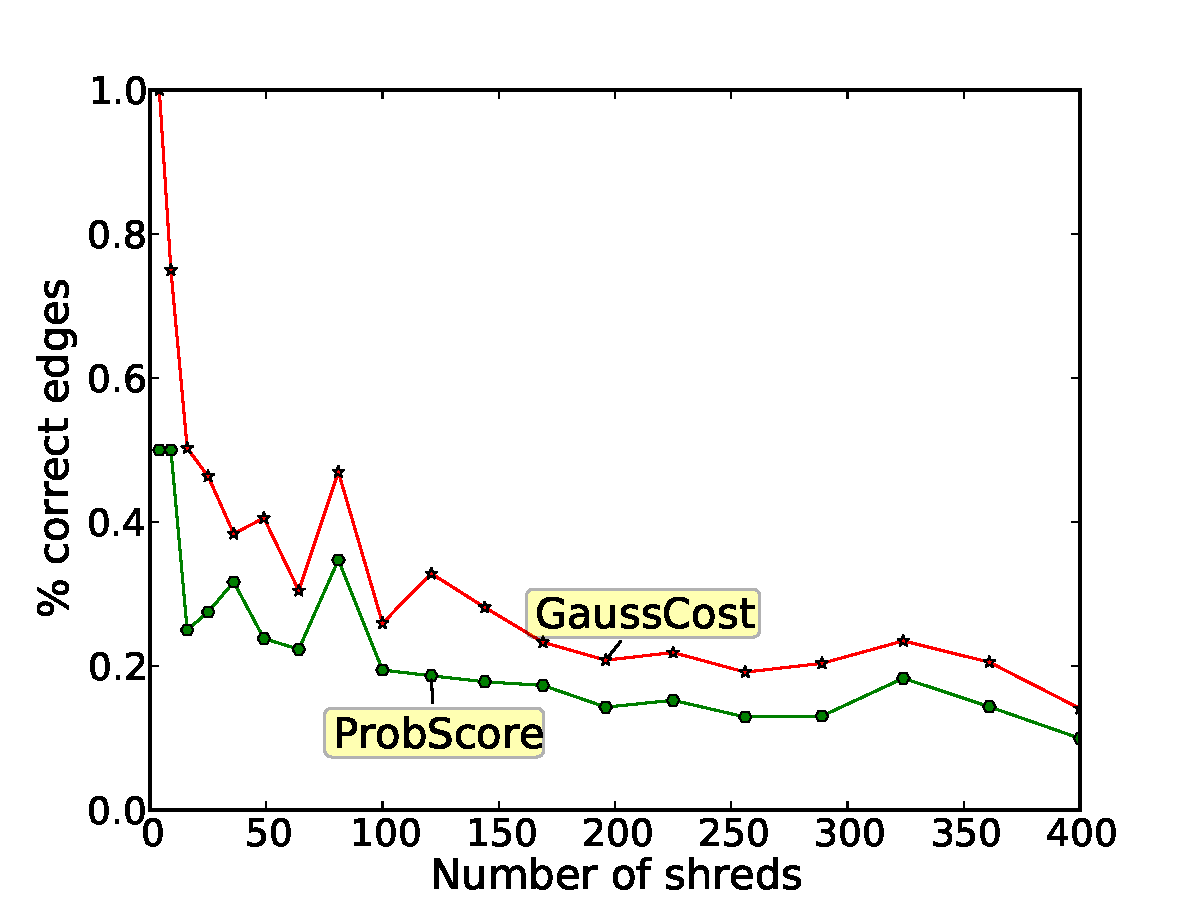
\includegraphics[width=\textwidth]{noise.pdf}
                \caption{10\% of bits are randomly flipped}
        \end{subfigure}
        ~ 
        \begin{subfigure}[b]{0.49\textwidth}
                \centering
                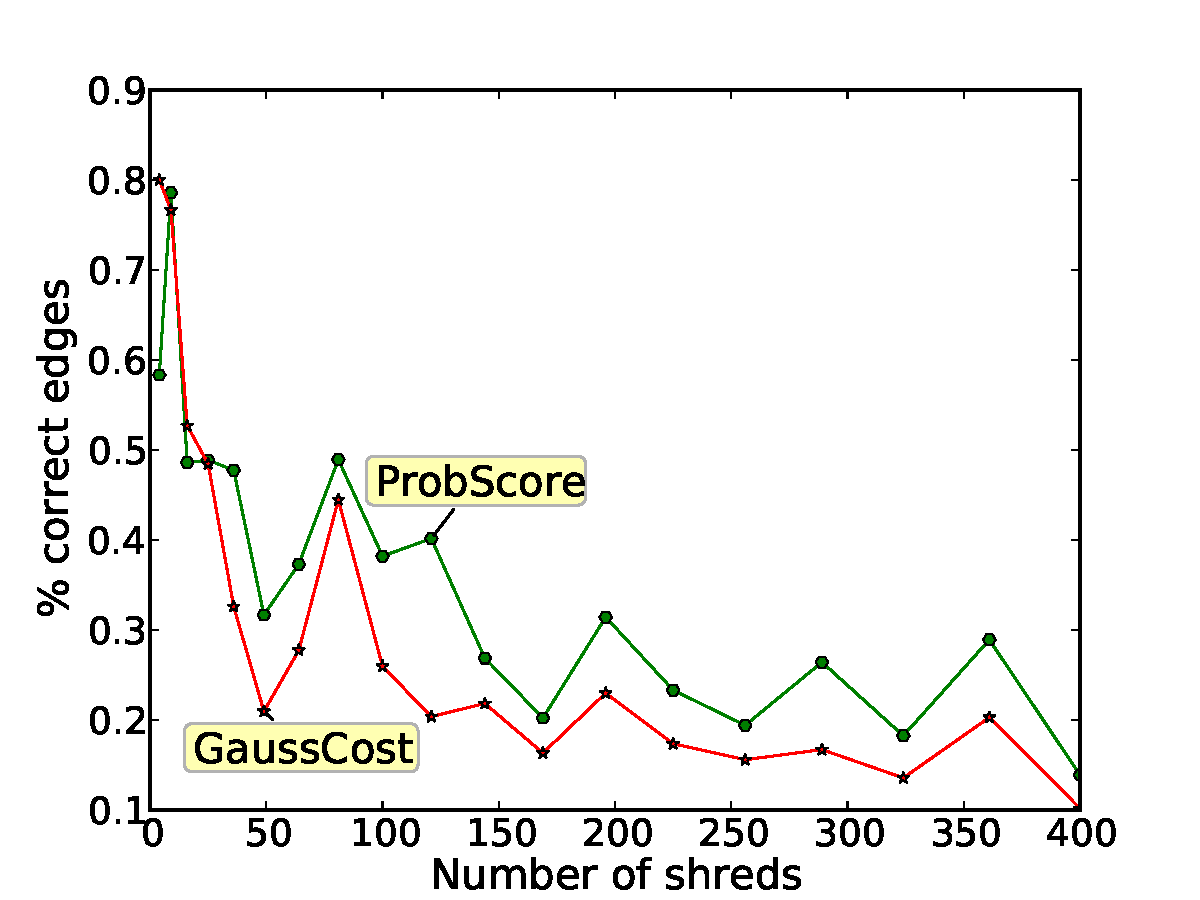
\includegraphics[width=\textwidth]{downsample.pdf}
                \caption{The image is downsampled by a factor of 1.5}
        \end{subfigure}
        ~ 
        \begin{subfigure}[b]{0.49\textwidth}
                \centering
                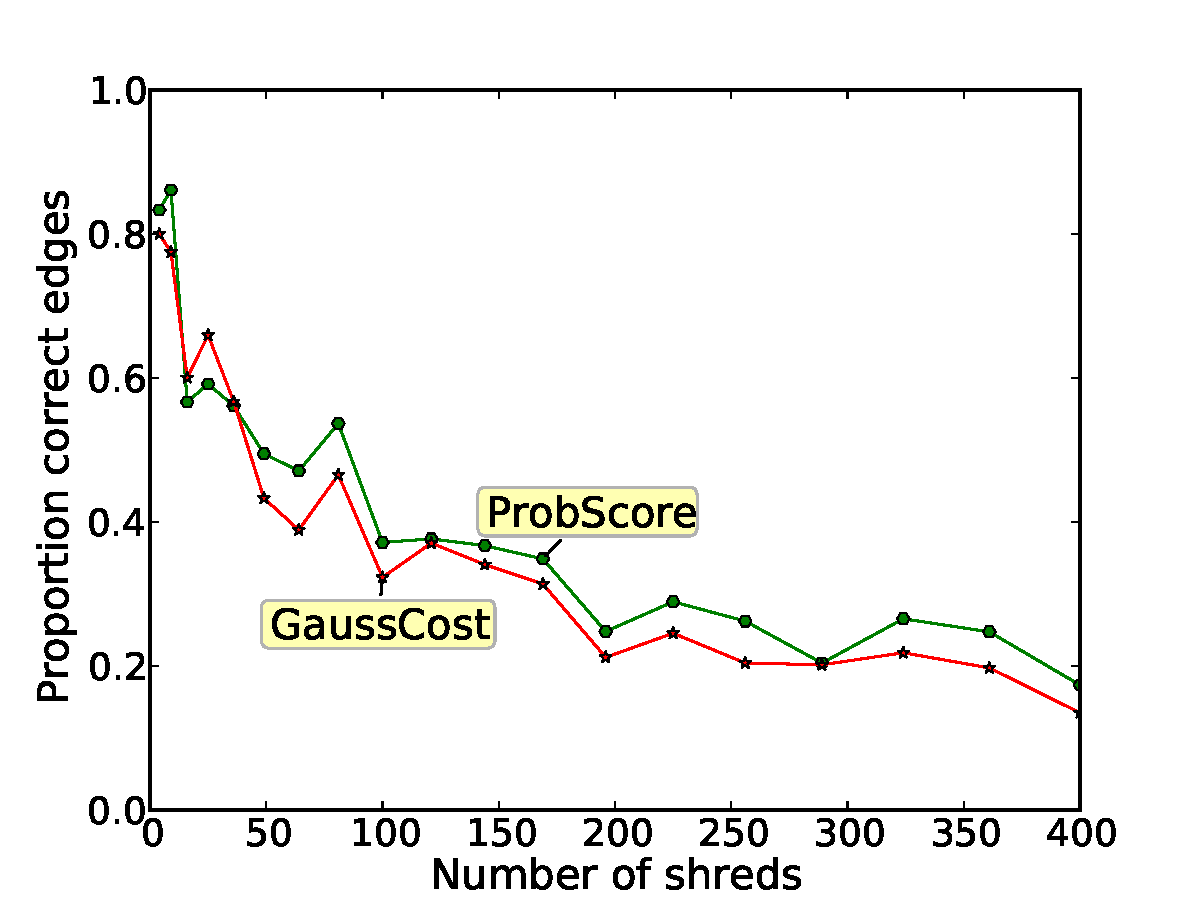
\includegraphics[width=\textwidth]{shuffle.pdf}
                \caption{Pixels are randomly shuffled to one of their neighbours}
        \end{subfigure}
        \caption{ProbScore outperforms the best Gaussian cost function on 3 out of 4 noise variants. The poor performance on case (b) is due to the simple probabilistic model not being able to cope well with completely random noise. However, this type of noise is less likely to be encountered than the other variants.}
        \label{fig:robComp}
\end{figure}

\section{Drawbacks}

Finally, we'll look at some of the flaws in the probabilistic scoring function and at some possible solutions.

\subsection{Uniformity assumption}
Learning a single set of conditional values of the form \(\Pr(p_i \mid C(p_i,E_x)) \), where the number of possible contexts $C(p_i,E_x)$ is small, implicitly makes the assumption that these conditional values are relatively uniform over the whole document. This is usually a reasonable assumption to make if the documents we're interested in are all text. However this assumption is certainly not always justified. Consider the document from Figure \ref{fig:tableText}. Here we can clearly see that there are two distinct regions, the text region and the table region. An algorithm which tries to fit a single valued model with a small context to this document cannot achieve very good results, because this document cannot be described well by such a model. The problem will only be compounded if we're looking at multiple shredded pages from possibly different documents.

\begin{figure}[h]
\centering
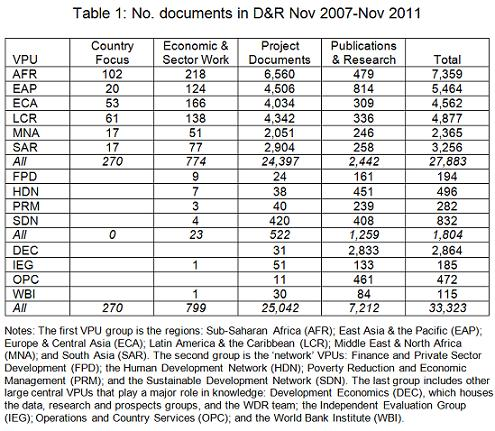
\includegraphics[width=10cm]{tableText}
\caption{A document in which the uniformity assumption is wrong.}
\label{fig:tableText}
\end{figure}

One solution here is to make the context complex enough to remove the uniformity assumption, by being able to tell between the different regions in the document. This could be done by using a significantly larger context size, or perhaps by using a different probabilistic model that takes higher level features into account (see also Section \ref{chap5NE}). A different approach would be to first split the shreds into categories and then learn a set of conditioned probabilities for every category. In theory this could also help reduce the problem size, by separating the documents into smaller uniform regions. However, avoiding overfitting might be difficult in this scenario. For instance, we wouldn't want the model to decide that every boldfaced piece of text belongs together in a separate uniform region.

\subsection{Lack of symmetry}
If \(E_x\) and \(E_y\) are two edges and \(E_x^{rot}\) and \(E_y^{rot}\) are the previous edges rotated by \(180^\circ\) then we might reasonably expect that \[\forall E_x \forall E_y \Pr(E_x,E_y) = \Pr(E_y^{rot},E_x^{rot})\] This would be a good property to have, since we are essentially comparing the exact same edge matching in both situations. However, the current probabilistic model offers no such guarantee. In particular the probabilistic model cannot guarantee that \(P(E_x,E_y) = P(E_y^{rot},E_x^{rot}) \) because it is not assured (and indeed quite unlikely) that enough data was present for these two conditional probabilities to have converged to the same value.

Depending on the situation this deficiency could be ignored. It is possible, however, that the search function being employed will assume the score to be symmetric. In that case, the best solution seems to be to calculate both \(\Pr(E_x,E_y)\) and  \(\Pr(E_y^{rot},E_x^{rot})\) and re-assign both probabilities to some number in between the 2 original probabilities (arguments could be made for either $min$, $max$ or $avg$). Care should be taken that this re-assignment is done before the normalization step, otherwise the values will no longer add up to 1.

\subsection{Ignoring non-edge information}
\label{chap5NE}
This problem is common to both the probabilistic score and all the cost functions presented above. It is also the hardest to fix. Figure \ref{fig:fakeMatch} shows an error made on a 5x5 cross-cut document. It is interesting to notice how even in a document cut into only 25 pieces such a convincing false match can occur. As the size of the shreds and therefore the amount of information available to our scoring function decreases further we can expect a huge number of such mistakes, making reconstruction of any non-trivial cross-cut document problematic.

\begin{figure}[h]
\centering
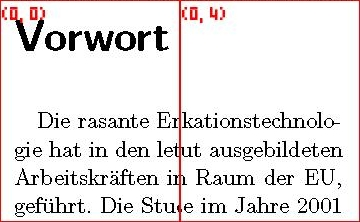
\includegraphics[width=0.6\textwidth]{conf.jpg}
\caption{An incorrect match that would be very difficult to detect by a cost/score function which only looks at the edge pixels}
\label{fig:fakeMatch}
\end{figure}

The solution here likely involves combining multiple scoring functions looking at different sets of features, both higher and lower level. Luckily, as mentioned above, the probabilistic score can easily accommodate any such scoring functions as long as they can express their result as a probability. One possible higher level scoring functions is discussed in Section \ref{chap4Mod}.

\section{Modularity}
\label{chap4Mod}

One of the big advantages of using a probabilistic scoring function is that this allows for very easy composition with any other probabilistic function. As a proof-of-concept implementation, we propose a very simple function, called ``RowScore", and show how it can be composed with the probabilistic scoring function.

``RowScore" is based on the idea that rows in neighbouring shreds should generally match. We identify all the rows in the shreds and, when looking at a potential shred match, sum up all the discrepancies between neighbouring rows. In order to formally define this sum, we specify a function $neighRow$ such that, if $A$ is a shred and $t$ is a y coordinate, then: \[neighRow(A,t) = \mbox{the y coordinate of the row in A closest to location t} \] If we also define $rows(A)$ to be a set of the y coordinates of all rows in shred $A$, the measure of how well shreds $A$ and $B$ match is then given by: \[RowDist(A,B) = \sum_{t \in rows(A)} |t - neighRow(B,t)| \] In order to translate this distance into a probability, we can make a simple Gaussian assumption. We want to assign the most probability mass to the case when the distance is $0$, so this is the mean of the distribution. Therefore the final form of ``RowScore" is\footnote{The variance of the normal distribution can be set empirically, but should take account of the size of the shreds. In experiments we have seen that the performance is not very sensitive to this value.}: \[ RowScore(A,B) = \frac{\displaystyle {e}^{-\frac{x^2}{2\sigma^2}}}{\sigma \sqrt{2\pi}} \]

Using the above method, we can give the probabilistic scoring function a small but consistent boost in performance, as shown in Figure \ref{fig:rowScore}.
\begin{figure}[h]
\centering
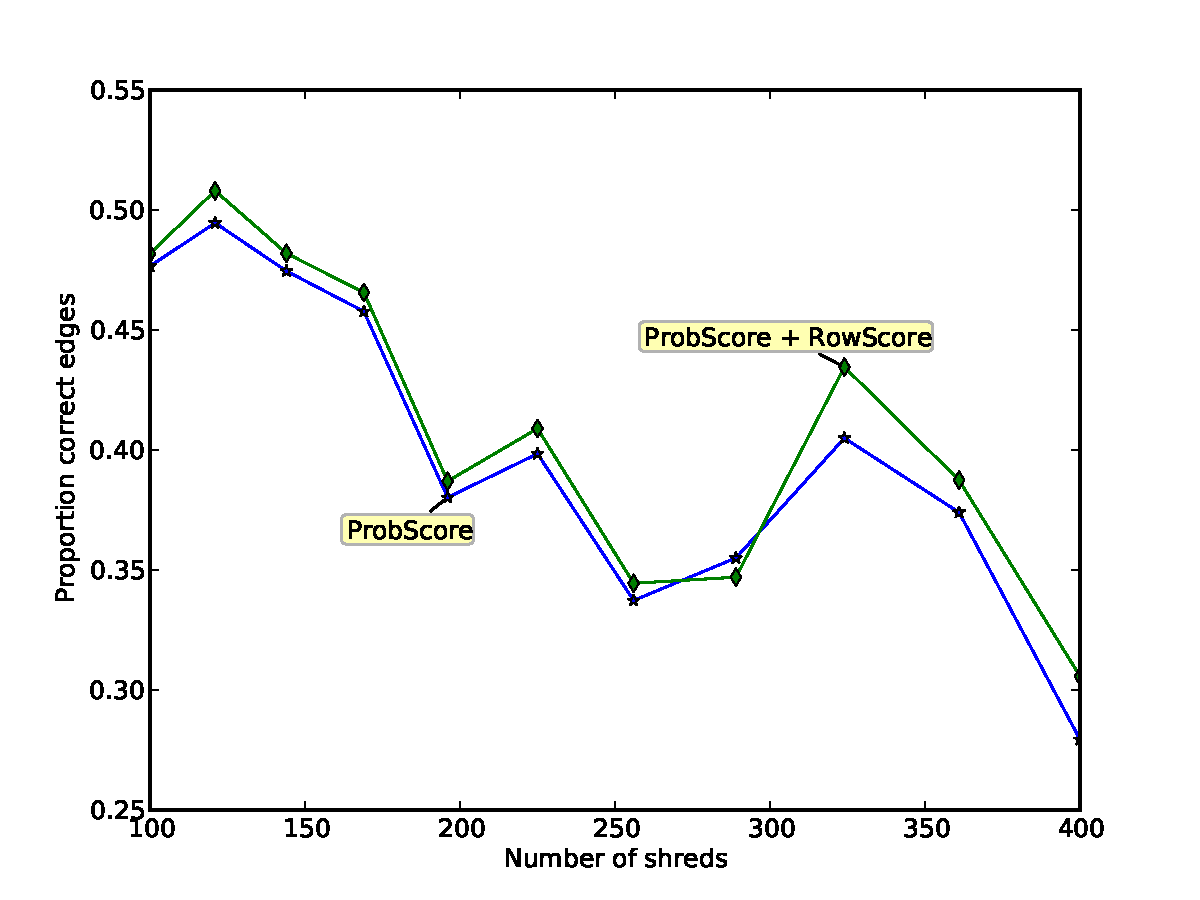
\includegraphics[width=0.95\textwidth]{rowScore.pdf}
\caption{Even the extremely simple ``RowScore" model gives a noticeable and consistent boost in performance to the probabilistic scoring function.}
\label{fig:rowScore}
\end{figure}
